\documentclass[aspectratio=1610]{beamer}
% \documentclass[handout]{beamer} % no animation version

% Theme and settings
\usetheme{Madrid}
\usecolortheme{seagull}
\usepackage{amsmath, amssymb}
\usepackage{listings}

\usepackage{xcolor}
\usepackage{tikz}
\usetikzlibrary{shapes.geometric, positioning, calc, patterns, patterns.meta, backgrounds}


\newcommand{\sssColor}{green}
\newcommand{\ssColor}{red}
\newcommand{\sColor}{blue}

\newlength{\y}
\newcommand{\width}{6mm}
\newcommand{\height}{3.3mm}

\newcommand{\vgap}{
    \addtolength{\y}{-\height}
    \addtolength{\y}{-1mm}
}
\newcommand{\vGap}{
    \addtolength{\y}{-\height}
    \addtolength{\y}{-3mm}
}

% Define TikZ styles for "XOR"
\tikzset{    
    % shape
    block_style/.style={minimum width = #1*\width, minimum height = \height, inner sep = 0pt, anchor = west},
    block/.style={draw, block_style = #1},
    inblock/.style={ultra thin, block = #1}, % dash pattern=on 1pt off 1pt, 
    zero_pad/.style={block_style = #1, gray},
    XOR/.style={draw, circle, minimum size=1.3*\height, 
        append after command={
            [shorten >=\pgflinewidth, shorten <=\pgflinewidth,]
            (\tikzlastnode.north) edge (\tikzlastnode.south)
            (\tikzlastnode.east) edge (\tikzlastnode.west)
        }
    },
    MULT/.style={draw, circle, minimum size=1.3*\height,
        append after command={
            [shorten >=\pgflinewidth, shorten <=\pgflinewidth]
            (\tikzlastnode.north west) edge (\tikzlastnode.south east)
            (\tikzlastnode.north east) edge (\tikzlastnode.south west)
        }
    },
    HMAC/.style={draw, ellipse, minimum width = \width, minimum height = \height, inner sep = 0pt, anchor = center},
    arrow/.style={->, shorten <= 1pt, shorten >= 2pt},
    arrowB/.style={->, shorten <= 2pt, shorten >= 4pt, color = lightgray},
    % display
    gray/.style={fill = gray, fill opacity=0.3},
    green/.style={fill = green, fill opacity=0.3},
    red/.style={fill = red, fill opacity=0.3},
    one/.style={pattern = north east lines, pattern color = \sColor},
    two/.style={pattern = north west lines, pattern color = \ssColor},
    three/.style={pattern = grid, pattern color = \sssColor},
}

\title{Sphinx Packets}
\subtitle{Decentralized Header Construction}
\author{Aurélien Chassagne}
\date{February 18, 2025} % \today

\begin{document}

% Title slide
\begin{frame}
\titlepage
\end{frame}

% Outline slide
% \begin{frame}{Outline}
% \tableofcontents
% \end{frame}

\scriptsize
\section{Original schema}
\begin{frame}{Mixnet}
    \centering
    \begin{figure}
        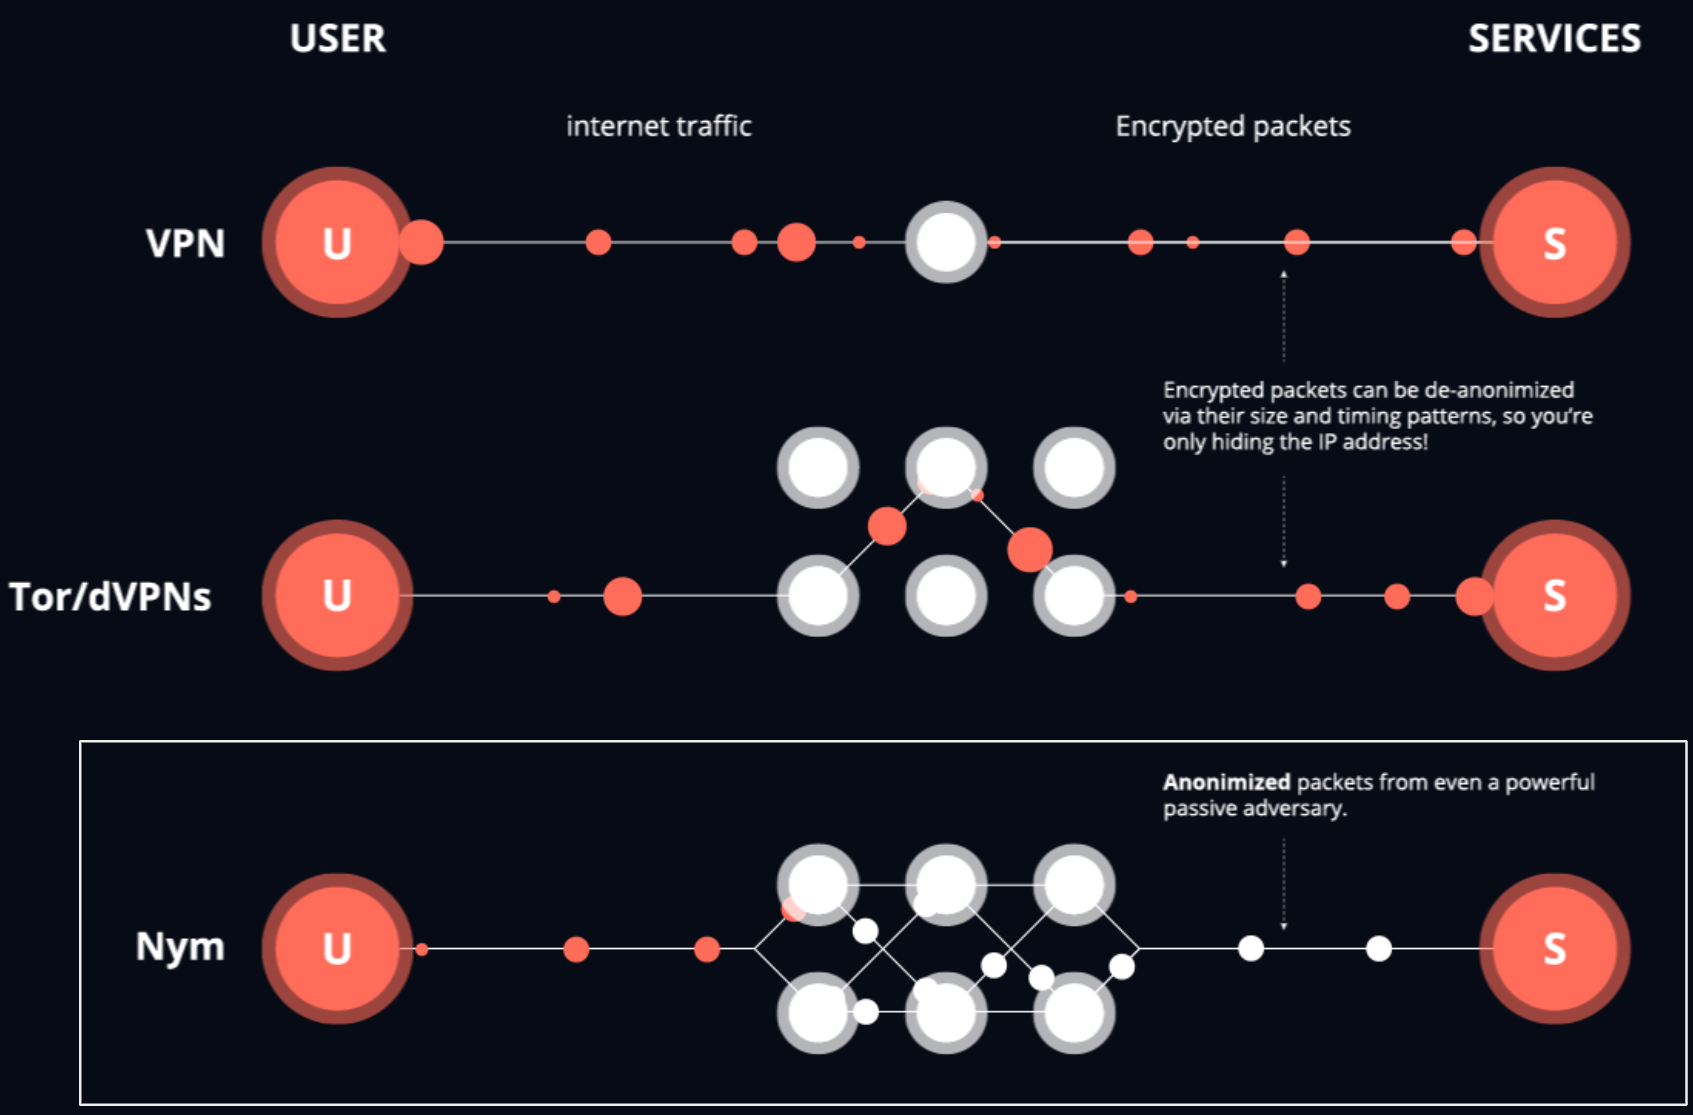
\includegraphics[width=0.8\linewidth]{Images/mixnet.png}
    \end{figure} 
\end{frame}

\begin{frame}{Schema overview}
    \centering
    \begin{figure}
        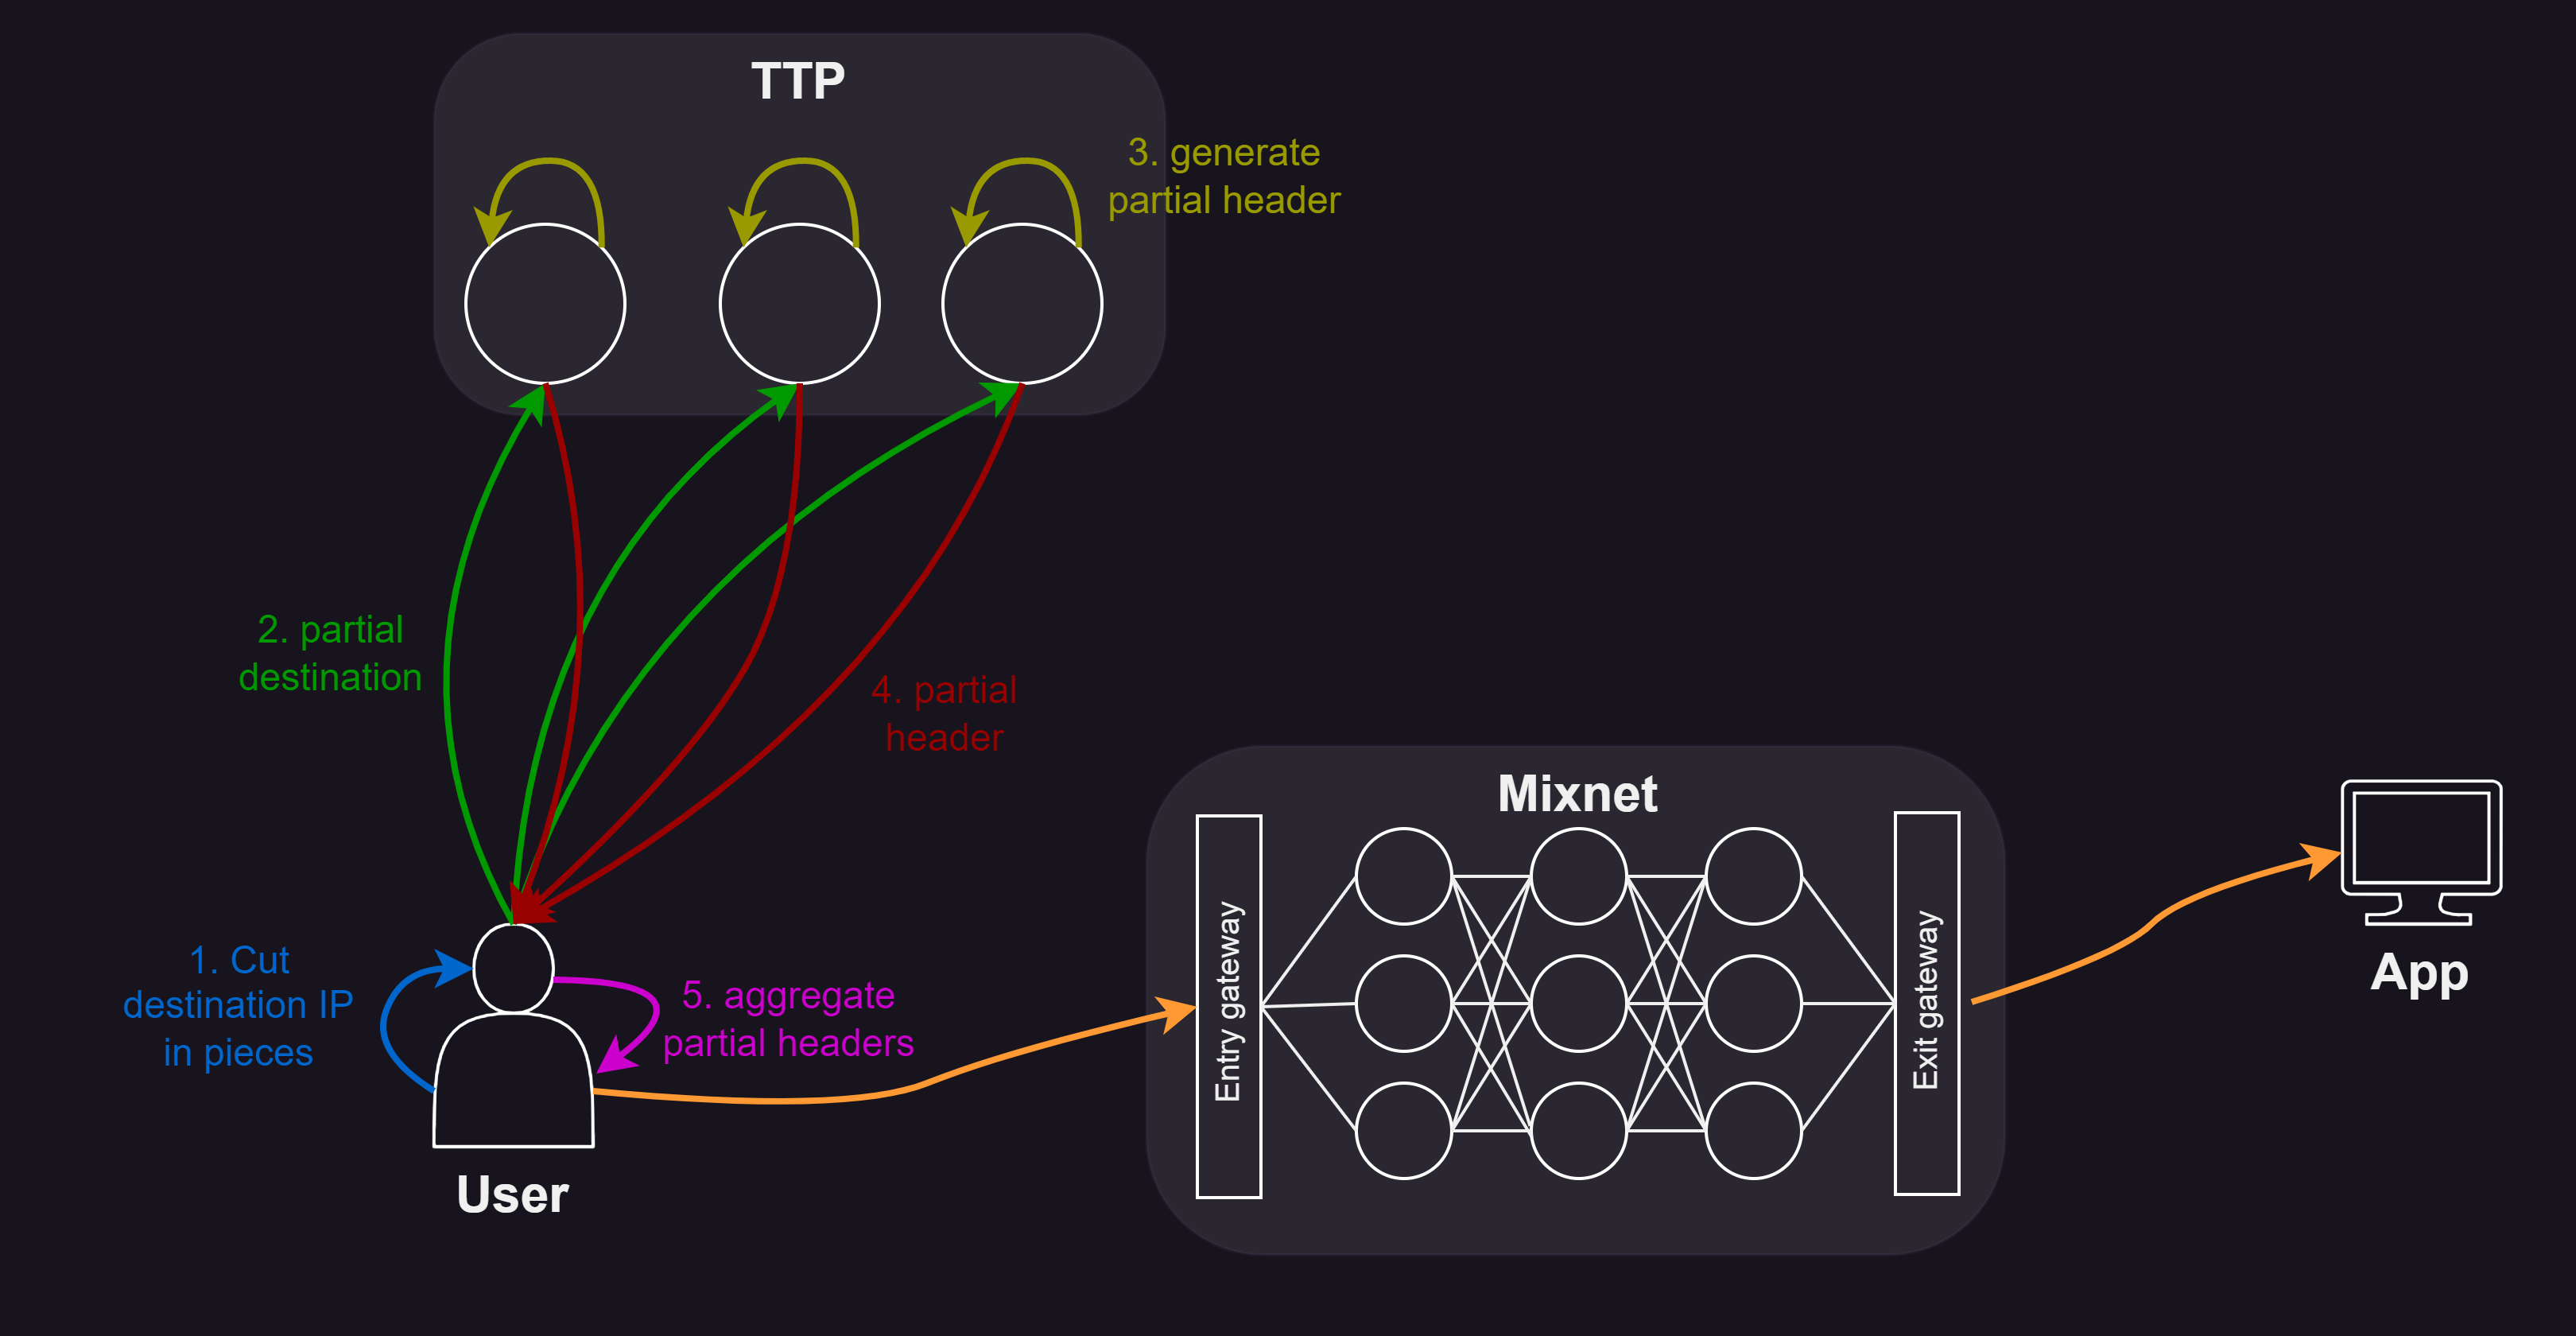
\includegraphics[width=\linewidth]{Images/sphinx_ttp.png}
    \end{figure}
\end{frame}

\begin{frame}{Desired properties}
    \begin{itemize}
        \setlength\itemsep{4mm}
        \onslide<1->
        \item {\normalsize Generic properties}
        \begin{itemize}
            \setlength\itemsep{2mm}
            \item {\color{lightgray}\textbf{\normalsize Correctness}: schema works without adversary}
            \item {\color{lightgray}\textbf{\normalsize Compactness}: Minimal overhead}
            \item {\color{lightgray}\textbf{\normalsize Efficiency}: Easy and fast to compute (e.g. XOR, hash, exponentiation,...)}
        \end{itemize}
        \onslide<2->
        \item {\normalsize Depends on the mixnode}
        \begin{itemize}
            \setlength\itemsep{2mm}\item {\color{olive}\textbf{\normalsize Forward / reply Undistinguishibility}: Cannot distinguish forward from reply packet}
            \item {\color{olive}\textbf{\normalsize Replay attack resistant:}: Cannot reused previous packet}    
        \end{itemize}
        \onslide<3->
        \item {\normalsize Depends on the header}
        \begin{itemize}
            \setlength\itemsep{2mm}
            \item {\color{olive}\textbf{\normalsize Integrity}: Maximum size path}
            \item {\color{orange}\textbf{\normalsize Wrap-resistance}: Unable to increase the intial path}
            \item {\color{red}\textbf{\normalsize Unlinkability}: Cannot link incoming and outgoing packet from a mixnode}
        \end{itemize}
    \end{itemize}
\end{frame}

\begin{frame}{Unlinkability compromised}
\begin{columns}
    \begin{column}{0.5\textwidth}
        \centering
        \vfill
        {\textbf{Original schema}}
        \vfill
        \begin{figure}
            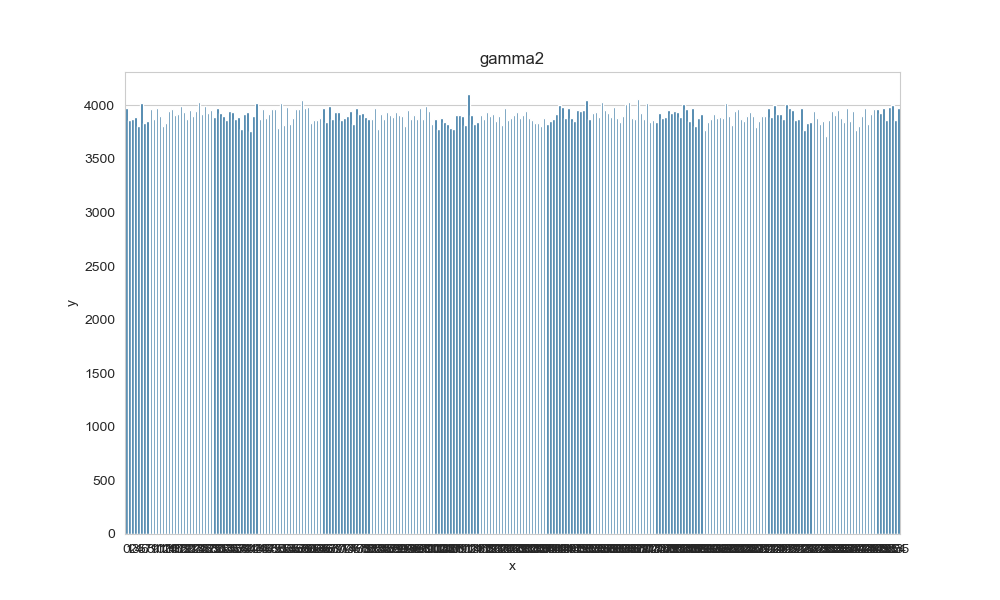
\includegraphics[scale=0.3]{Images/res/origin_gamma2.png}
        \end{figure}
    \end{column} 
    \vrule
    \begin{column}{0.5\textwidth}
        \centering
        \vfill
        {\textbf{My schema}}
        \vfill
        \begin{figure}
            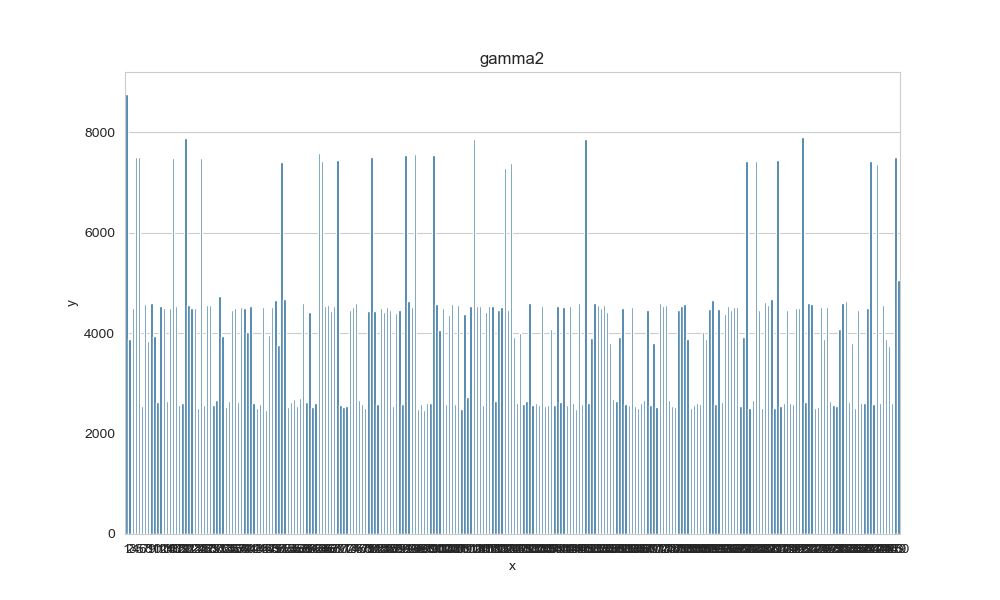
\includegraphics[scale=0.3]{Images/res/test_gamma2.png}
        \end{figure}
    \end{column}
\end{columns}
\end{frame}

\begin{frame}{Unlinkability compromised}
\centering
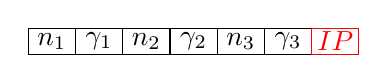
\begin{tikzpicture}
    \node (b1) [block=5]  at (2*\width, 0) {};
    \node (n1) [block=1]  at (0, 0) {$n_1$}; 
    \node (y1) [block=1]  at (\width, 0) {$\gamma_1$}; 
    \node [block=1] at (2*\width, 0) {$n_2$}; 
    \node [block=1] at (3*\width, 0) {$\gamma_2$}; 
    \node [block=1] at (4*\width, 0) {$n_3$}; 
    \node [block=1] at (5*\width, 0) {$\gamma_3$}; 
    \node [block=1, color=red] at (6*\width, 0) {$IP$};
\end{tikzpicture}
\begin{figure}
    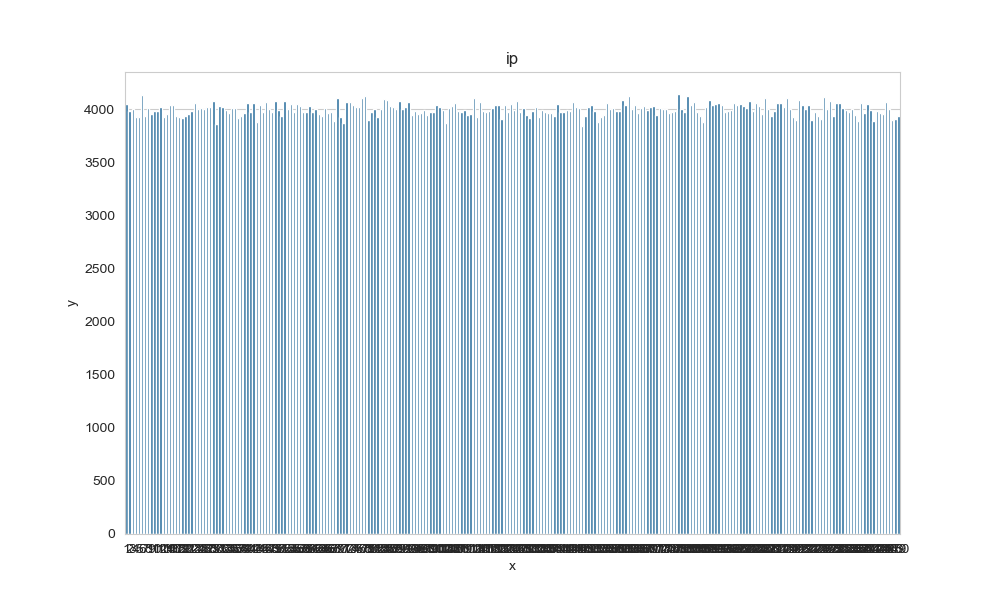
\includegraphics[width=0.9\linewidth]{Images/res/test_ip.png}
\end{figure}
\end{frame}

\begin{frame}{Unlinkability compromised}
    \centering
    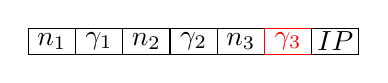
\begin{tikzpicture}
        \node (b1) [block=5]  at (2*\width, 0) {};
        \node (n1) [block=1]  at (0, 0) {$n_1$}; 
        \node (y1) [block=1]  at (\width, 0) {$\gamma_1$}; 
        \node [block=1] at (2*\width, 0) {$n_2$}; 
        \node [block=1] at (3*\width, 0) {$\gamma_2$}; 
        \node [block=1] at (4*\width, 0) {$n_3$}; 
        \node [block=1, color=red] at (5*\width, 0) {$\gamma_3$}; 
        \node [block=1] at (6*\width, 0) {$IP$};
    \end{tikzpicture}
    \begin{figure}
        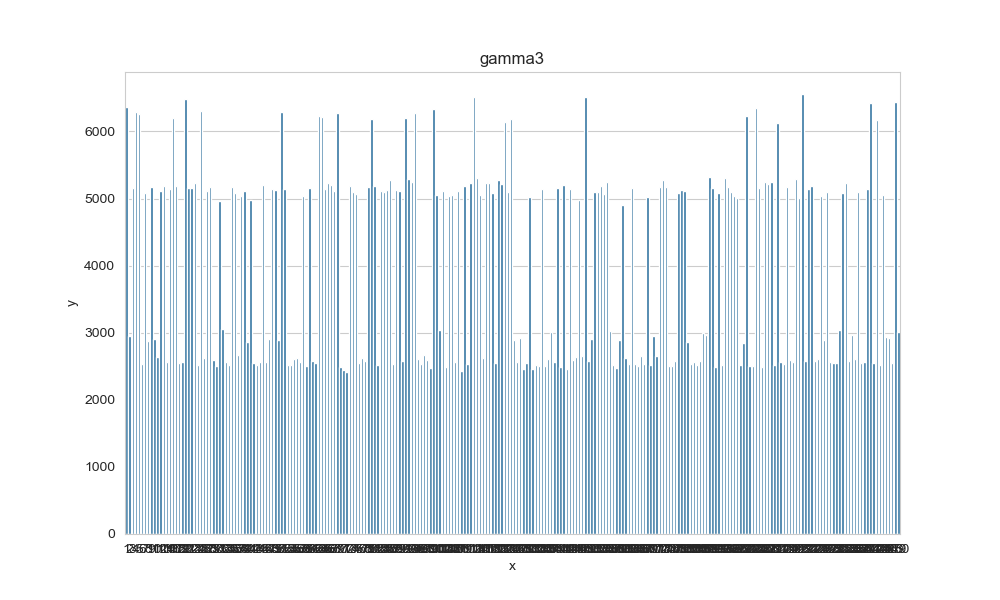
\includegraphics[width=0.9\linewidth]{Images/res/test_gamma3.png}
    \end{figure}
\end{frame}

\begin{frame}{Unlinkability compromised}
    \centering
    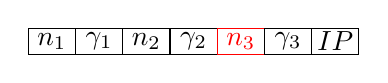
\begin{tikzpicture}
        \node (b1) [block=5]  at (2*\width, 0) {};
        \node (n1) [block=1]  at (0, 0) {$n_1$}; 
        \node (y1) [block=1]  at (\width, 0) {$\gamma_1$}; 
        \node [block=1] at (2*\width, 0) {$n_2$}; 
        \node [block=1] at (3*\width, 0) {$\gamma_2$}; 
        \node [block=1, color=red] at (4*\width, 0) {$n_3$}; 
        \node [block=1] at (5*\width, 0) {$\gamma_3$}; 
        \node [block=1] at (6*\width, 0) {$IP$};
    \end{tikzpicture}
    \begin{figure}
        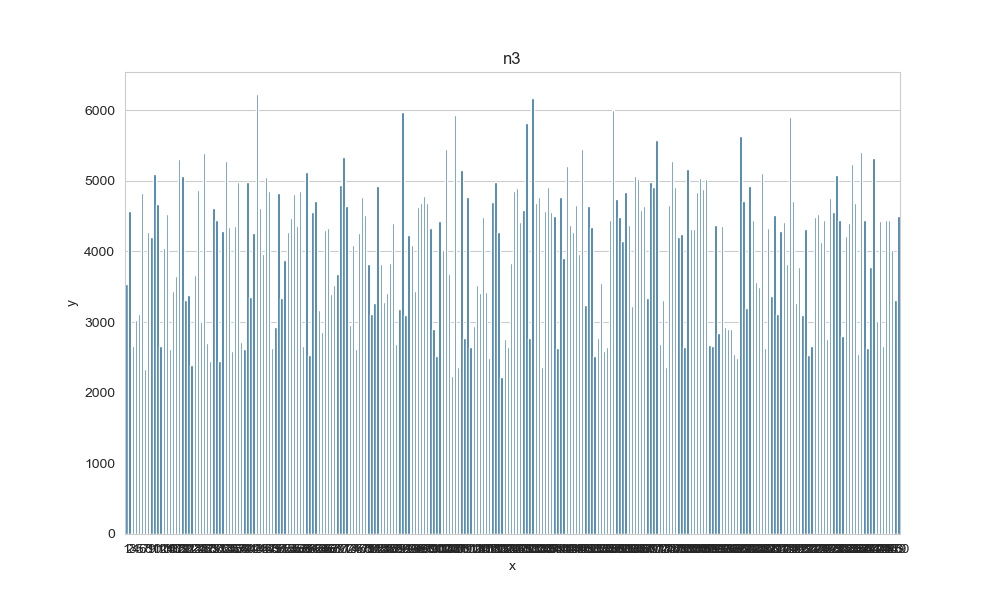
\includegraphics[width=0.9\linewidth]{Images/res/test_n3.png}
    \end{figure}
\end{frame}

\begin{frame}{Unlinkability compromised}
    \centering
    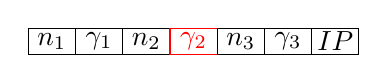
\begin{tikzpicture}
        \node (b1) [block=5]  at (2*\width, 0) {};
        \node (n1) [block=1]  at (0, 0) {$n_1$}; 
        \node (y1) [block=1]  at (\width, 0) {$\gamma_1$}; 
        \node [block=1] at (2*\width, 0) {$n_2$}; 
        \node [block=1, color=red] at (3*\width, 0) {$\gamma_2$}; 
        \node [block=1] at (4*\width, 0) {$n_3$}; 
        \node [block=1] at (5*\width, 0) {$\gamma_3$}; 
        \node [block=1] at (6*\width, 0) {$IP$};
    \end{tikzpicture}
    \begin{figure}
        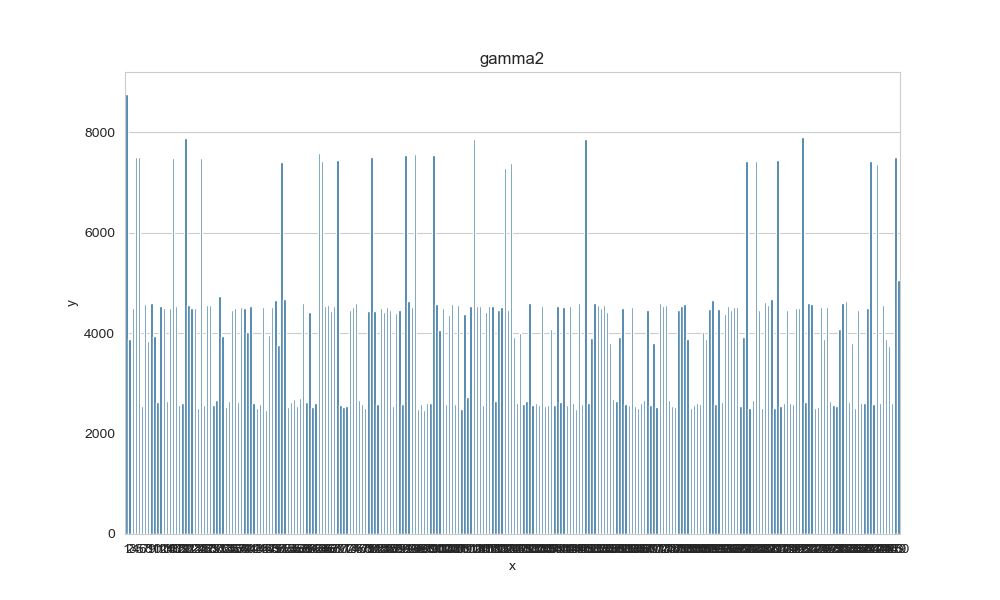
\includegraphics[width=0.9\linewidth]{Images/res/test_gamma2.png}
    \end{figure}
\end{frame}

\begin{frame}{Unlinkability compromised}
    \centering
    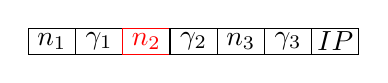
\begin{tikzpicture}
        \node (b1) [block=5]  at (2*\width, 0) {};
        \node (n1) [block=1]  at (0, 0) {$n_1$}; 
        \node (y1) [block=1]  at (\width, 0) {$\gamma_1$}; 
        \node [block=1, color=red] at (2*\width, 0) {$n_2$}; 
        \node [block=1] at (3*\width, 0) {$\gamma_2$}; 
        \node [block=1] at (4*\width, 0) {$n_3$}; 
        \node [block=1] at (5*\width, 0) {$\gamma_3$}; 
        \node [block=1] at (6*\width, 0) {$IP$};
    \end{tikzpicture}
    \begin{figure}
        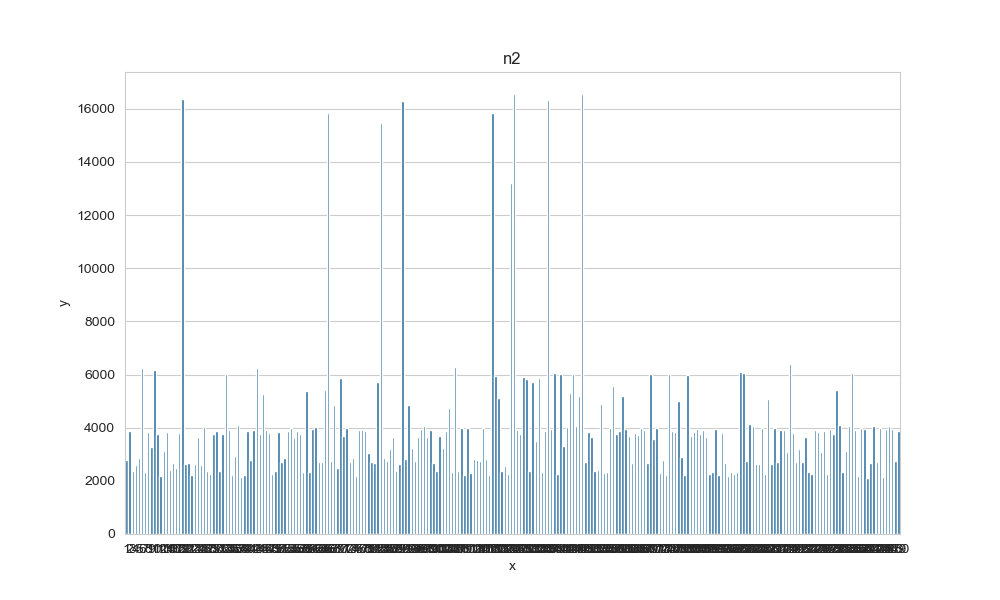
\includegraphics[width=0.9\linewidth]{Images/res/test_n2.png}
    \end{figure}
\end{frame}

\begin{frame}{Unlinkability compromised}
    \centering
    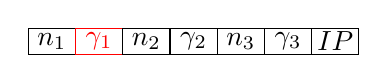
\begin{tikzpicture}
        \node (b1) [block=5]  at (2*\width, 0) {};
        \node (n1) [block=1]  at (0, 0) {$n_1$}; 
        \node (y1) [block=1, color=red]  at (\width, 0) {$\gamma_1$}; 
        \node [block=1] at (2*\width, 0) {$n_2$}; 
        \node [block=1] at (3*\width, 0) {$\gamma_2$}; 
        \node [block=1] at (4*\width, 0) {$n_3$}; 
        \node [block=1] at (5*\width, 0) {$\gamma_3$}; 
        \node [block=1] at (6*\width, 0) {$IP$};
    \end{tikzpicture}
    \begin{figure}
        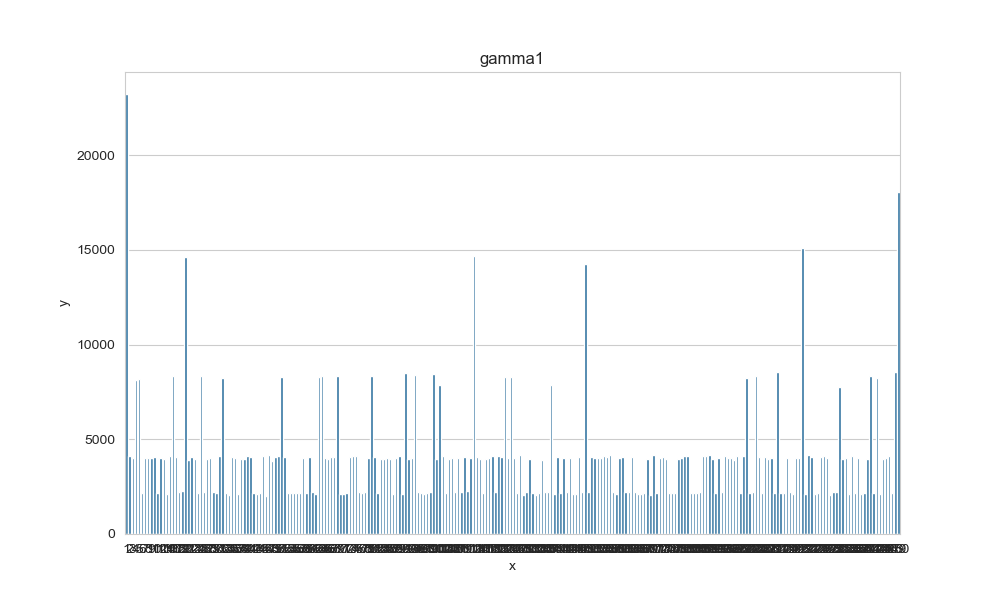
\includegraphics[width=0.9\linewidth]{Images/res/test_gamma1.png}
    \end{figure}
\end{frame}

\begin{frame}{Unlinkability compromised}
    \centering
    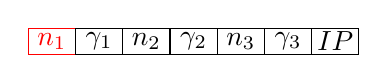
\begin{tikzpicture}
        \node (b1) [block=5]  at (2*\width, 0) {};
        \node (n1) [block=1, color=red]  at (0, 0) {$n_1$}; 
        \node (y1) [block=1]  at (\width, 0) {$\gamma_1$}; 
        \node [block=1] at (2*\width, 0) {$n_2$}; 
        \node [block=1] at (3*\width, 0) {$\gamma_2$}; 
        \node [block=1] at (4*\width, 0) {$n_3$}; 
        \node [block=1] at (5*\width, 0) {$\gamma_3$}; 
        \node [block=1] at (6*\width, 0) {$IP$};
    \end{tikzpicture}
    \begin{figure}
        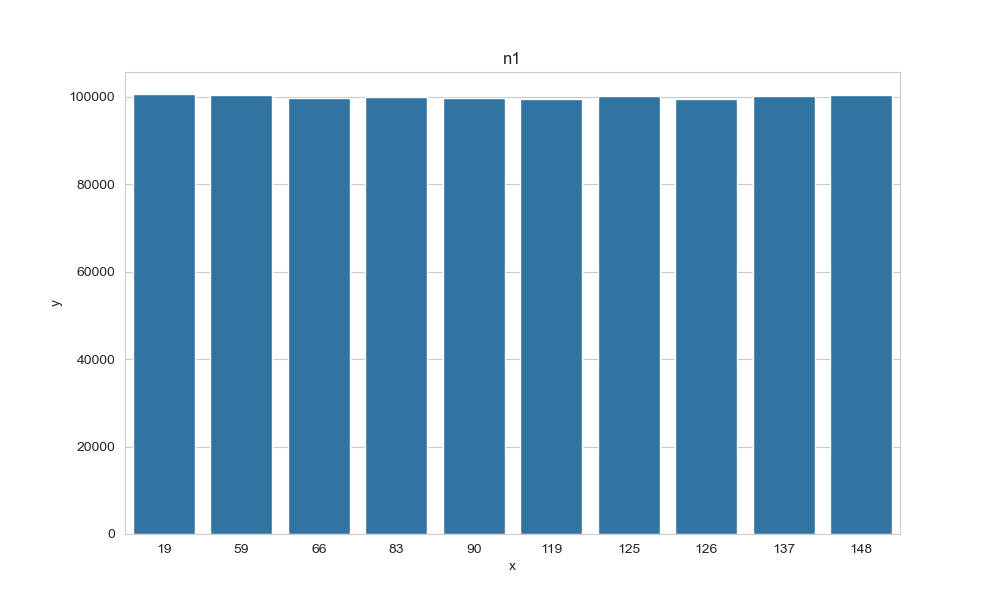
\includegraphics[width=0.9\linewidth]{Images/res/test_n1.png}
    \end{figure}
\end{frame}
\begin{frame}{Reproduce article's figure}

\begin{columns} 
\begin{column}{0.5\textwidth}
    \begin{figure}
        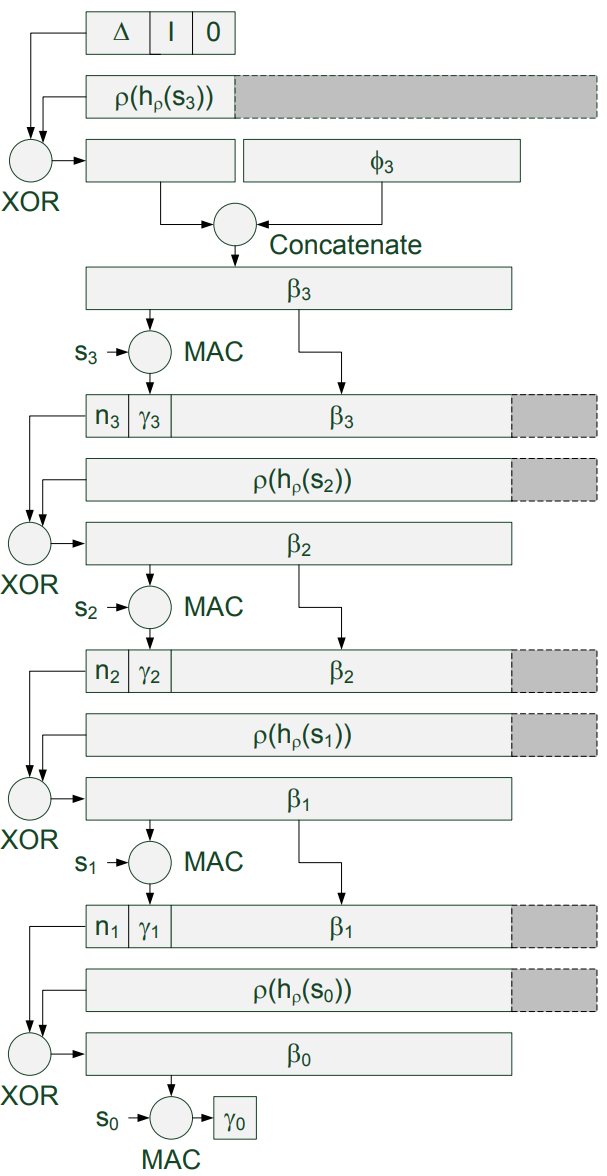
\includegraphics[scale=0.19]{Images/origin_beta_construction.png}
    \end{figure}
\end{column}

\vrule

\begin{column}{0.5\textwidth}\onslide<2->
\centering
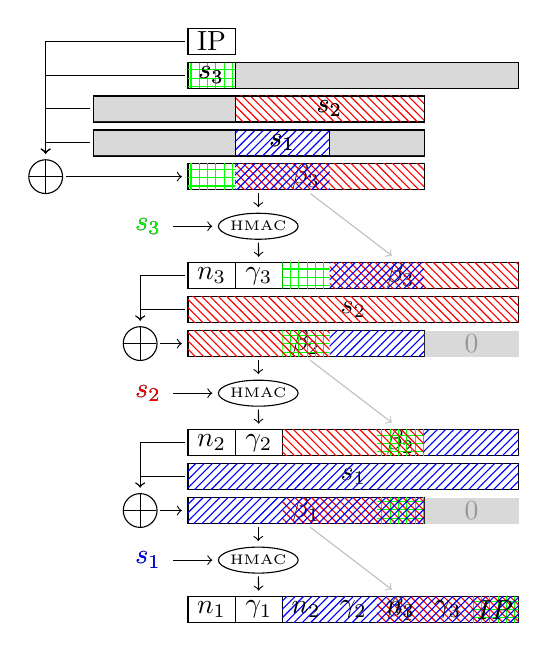
\begin{tikzpicture}
    \setlength{\y}{0cm}

    \node (ip) [block=1] at (0, \y) {IP};
    \vgap
    \node (s3_) [block=7] at (0, \y) {};
    \node [inblock=1] at (0, \y) {$s_3$};
    \onslide<3-> {\node [inblock=1, three] at (0, \y) {$s_3$};}
    \node [inblock=6, gray] at (\width, \y) {}; 
    \vgap
    \node (s2_) [block=7] at (- 2*\width, \y) {};
    \node [inblock=3, gray] at (- 2*\width, \y) {}; 
    \node [inblock=4] at (3*\width - 2*\width, \y) {$s_2$};
    \onslide<3-> {\node [inblock=4, two] at (3*\width - 2*\width, \y) {$s_2$};}
    \vgap
    \node (s1_) [block=7] at (- 2*\width, \y) {};
    \node [inblock=3, gray] at (- 2*\width, \y) {}; 
    \node [inblock=2] at (3*\width - 2*\width, \y) {$s_1$};
    \onslide<3-> {\node [inblock=2, one] at (3*\width - 2*\width, \y) {$s_1$};}
    \node [inblock=2, gray] at (5*\width - 2*\width, \y) {};
    \vgap 
    \node (B3) [block=5] at (0, \y) {$\beta_3$}; 
    \onslide<3-> {
        \node [block_style=1, three] at (0, \y) {}; 
        \node [block_style=4, two] at (\width, \y) {}; 
        \node [block_style=2, one] at (\width, \y) {}; 
    }

    \node (xor3) [XOR] at (-3*\width, \y) {}; 
    \vGap
    \node (hmac3) [HMAC] at (1.5*\width, \y) {\tiny HMAC};
    \vGap
 
    \node (n3) [block=1] at (0, \y) {$n_3$}; 
    \node (y3) [block=1] at (\width, \y) {$\gamma_3$}; 
    \node (b3) [block=5] at (2*\width, \y) {$\beta_3$};
    \onslide<4-> {
        \node [block_style=1, three] at (2*\width, \y) {}; 
        \node [block_style=4, two] at (3*\width, \y) {}; 
        \node [block_style=2, one] at (3*\width, \y) {}; 
    } 
    \vgap
    \node (s2) [block=7] at (0, \y) {$s_2$};
    \onslide<5-> {\node [block_style=7, two] at (0, \y) {};}
    \vgap
    \node (B2) [block=5] at (0, \y) {$\beta_2$}; 
    \onslide<6-> {
        \node [block_style=1, three] at (2*\width, \y) {}; 
        \node [block_style=3, two] at (0*\width, \y) {}; 
        \node [block_style=2, one] at (3*\width, \y) {};
    } 
    \node (zero2) [zero_pad=2] at (5*\width, \y) {0}; 

    \node (xor2) [XOR] at (-\width, \y) {}; 
    \vGap
    \node (hmac2) [HMAC] at (1.5*\width, \y) {\tiny HMAC};
    \vGap

    \node (n2) [block=1] at (0, \y) {$n_2$}; 
    \node (y2) [block=1] at (\width, \y) {$\gamma_2$}; 
    \node (b2) [block=5] at (2*\width, \y) {$\beta_2$}; 
    \onslide<7-> {
        \node [block_style=1, three] at (4*\width, \y) {}; 
        \node [block_style=3, two] at (2*\width, \y) {}; 
        \node [block_style=2, one] at (5*\width, \y) {}; 
    } 
    \vgap
    \node (s1) [block=7] at (0, \y) {$s_1$};
    \onslide<8-> {\node [block_style=7, one] at (0, \y) {};}
    \vgap
    \node (B1) [block=5] at (0, \y) {$\beta_1$};
    \onslide<9-> {
        \node [block_style=1, three] at (4*\width, \y) {}; 
        \node [block_style=3, two] at (2*\width, \y) {}; 
        \node [block_style=5, one] at (0*\width, \y) {}; 
    } 
    \node (zero1) [zero_pad=2]  at (5*\width, \y) {0}; 

    \node (xor1) [XOR]  at (-\width, \y) {}; 
    \vGap
    \node (hmac1) [HMAC]  at (1.5*\width, \y) {\tiny HMAC};
    \vGap

    \node (n1) [block=1]  at (0, \y) {$n_1$}; 
    \node (y1) [block=1]  at (\width, \y) {$\gamma_1$}; 
    \onslide<1-9> {
        \node (b1) [block=5]  at (2*\width, \y) {$\beta_1$};
        % \node [block_style=1, three] at (6*\width, \y) {}; 
        % \node [block_style=3, two] at (4*\width, \y) {}; 
        % \node [block_style=5, one] at (2*\width, \y) {}; 
    }
    \onslide<10-> {
        \node (b1) [block=5]  at (2*\width, \y) {};
        \node [block_style=1, three] at (6*\width, \y) {}; 
        \node [block_style=3, two] at (4*\width, \y) {}; 
        \node [block_style=5, one] at (2*\width, \y) {}; 
        \node [block_style=1] at (2*\width, \y) {$n_2$}; 
        \node [block_style=1] at (3*\width, \y) {$\gamma_2$}; 
        \node [block_style=1] at (4*\width, \y) {$n_3$}; 
        \node [block_style=1] at (5*\width, \y) {$\gamma_3$}; 
        \node [block_style=1] at (6*\width, \y) {$IP$};
    }  

    %% XOR ARROWS %%
    % 3
    \draw[arrow] (ip.west) -- ++(-3*\width, 0) -- (xor3.north);
    \draw[arrow] (s3_.west) -- ++(-3*\width, 0) -- (xor3.north);
    \draw[arrow] (s2_.west) -- ++(-\width, 0) -- (xor3.north);
    \draw[arrow] (s1_.west) -- ++(-\width, 0) -- (xor3.north);
    \draw[arrow] (xor3.east) -- (B3.west);
    % 2
    \draw[arrow] (n3.west) -- ++(-\width, 0) -- (xor2.north);
    \draw[arrow] (s2.west) -- ++(-\width, 0) -- (xor2.north);
    \draw[arrow] (xor2.east) -- (B2.west);
    % 1
    \draw[arrow] (n2.west) -- ++(-\width, 0) -- (xor1.north);
    \draw[arrow] (s1.west) -- ++(-\width, 0) -- (xor1.north);
    \draw[arrow] (xor1.east) -- (B1.west);

    %% HMAC ARROWS %%
    % 3
    \node[left=\width of hmac3] (input_hmac3) {$s_3$};
    \onslide<4-> {\node[left=\width of hmac3] (input_hmac3) {\color{\sssColor}$s_3$};}
    \draw[arrow] (input_hmac3) -- (hmac3.west);
    \draw[arrow] (B3.south -| 1.5*\width, 0) -- (hmac3.north);
    \draw[arrow] (hmac3.south) -- (y3.north);
    % 2
    \node[left=\width of hmac2] (input_hmac2) {$s_2$};
    \onslide<7-> {\node[left=\width of hmac2] (input_hmac2) {\color{\ssColor}$s_2$};}
    \draw[arrow] (input_hmac2) -- (hmac2.west);
    \draw[arrow] (B2.south -| 1.5*\width, 0) -- (hmac2.north);
    \draw[arrow] (hmac2.south) -- (y2.north);
    % 1
    \node[left=\width of hmac1] (input_hmac1) {$s_1$};
    \onslide<10-> {\node[left=\width of hmac1] (input_hmac1) {\color{\sColor}$s_1$};}
    \draw[arrow] (input_hmac1) -- (hmac1.west);
    \draw[arrow] (B1.south -| 1.5*\width, 0) -- (hmac1.north);
    \draw[arrow] (hmac1.south) -- (y1.north);

    %% BETA ARROWS %%
    % 3
    \draw[arrowB] (B3.south) -- (b3.north);
    % 2
    \draw[arrowB] (B2.south) -- (b2.north);
    % 1
    \draw[arrowB] (B1.south) -- (b1.north);

\end{tikzpicture}
\end{column}

\end{columns}
\end{frame}
\begin{frame}{Adapting HMAC}

\begin{columns} 
\onslide<2->  
\begin{column}{0.5\textwidth}
    {\small \textbf{Main problem:} Decentralizing a \textbf{\color{red}Hash} ?} \newline

    \begin{itemize}
        \setlength\itemsep{2mm}
        \onslide<3->
        \item Need \textbf{homomorphic properties} \newline 
        to split computation and aggregate results.
        \onslide<4->
        \item Secure homomorphic hash \textbf{seems impractical} \newline
        (no promising solutions found).
        \onslide<5->
        \item Exploring \textbf{homomorphic encryption} as an alternative.
        \only<6> {
            \begin{enumerate}\scriptsize
                \setlength\itemsep{3mm}
                \item \textbf{RSA}
                \item \textbf{ElGamal}
                \item \textbf{Paillier}
            \end{enumerate}
        } \only<9> {
            \begin{enumerate}\scriptsize
                \setlength\itemsep{3mm}
                \item \textbf{RSA}\vspace{2mm}\newline
                $\begin{aligned}
                    {\mathcal {E}}(m_{1}) \cdot {\mathcal {E}}(m_{2})
                    &=m_{1}^{e}m_{2}^{e}\;{\bmod {\;}}n\\[6pt]
                    &=(m_{1}m_{2})^{e}\;{\bmod {\;}}n\\[6pt]
                    &={\mathcal {E}}(m_{1}\cdot m_{2})
                \end{aligned}$
                \item \textbf{ElGamal}
                \item \textbf{Paillier}
            \end{enumerate}
        } \only<8> {
            \begin{enumerate}\scriptsize
                \setlength\itemsep{3mm}
                \item \textbf{RSA}
                \item \textbf{ElGamal}\vspace{2mm}\newline
                $\begin{aligned}
                    {\mathcal {E}}(m_{1}) \cdot {\mathcal {E}}(m_{2}) 
                    &=({\color{orange}g^{r_{1}},}\; m_{1}\cdot h^{r_{1}})({\color{orange}g^{r_{2}},}\; m_{2}\cdot h^{r_{2}})\\[6pt]
                    &=({\color{orange}g^{r_{1}+r_{2}},}\; (m_{1}\cdot m_{2})h^{r_{1}+r_{2}})\\[6pt]
                    &={\mathcal {E}}(m_{1}\cdot m_{2})
                \end{aligned}$
                \item \textbf{Paillier}
            \end{enumerate}\vspace{4mm}
            \textbf{\color{orange}Limitation:} Increase ciphertext size...
        } \only<7> {
            \begin{enumerate}\scriptsize
                \setlength\itemsep{3mm}
                \item \textbf{RSA}
                \item \textbf{ElGamal}
                \item \textbf{Paillier}\vspace{2mm}\newline
                $\begin{aligned}
                    {\mathcal {E}}(m_{1}) {\color{red}\cdot} {\mathcal {E}}(m_{2})
                    &=(g^{m_{1}}r_{1}^{n})(g^{m_{2}}r_{2}^{n})\;{\bmod {\;}}n^{2}\\[6pt]
                    &=g^{m_{1}+m_{2}}(r_{1}r_{2})^{n}\;{\bmod {\;}}n^{2}\\[6pt]
                    &={\mathcal {E}}(m_{1} {\color{red}+} m_{2}).
                \end{aligned}$
            \end{enumerate}\vspace{4mm}
            \textbf{\color{red}Problem:} Mix of different operations... order matters!
        } \only<10> {
            \begin{enumerate}\scriptsize
                \setlength\itemsep{3mm}
                \item \textbf{RSA}
                \item \textbf{ElGamal}
                \item \textbf{Paillier}
            \end{enumerate}
        }
        \end{itemize}\vspace{5mm}
        \only<10> {
            \small \textbf{Selected solution: {\color{green}RSA} for integrity tag}\vspace{4mm}\newline
            \tiny
            \textbf{NB:} $s_i$ is different for each TTP but RSA required the same $e$...\newline
            Thus, create a new shared secret $s'_i$ common to all TTP
        }
\end{column}

\onslide<1->
\begin{column}{0.5\textwidth}
\centering
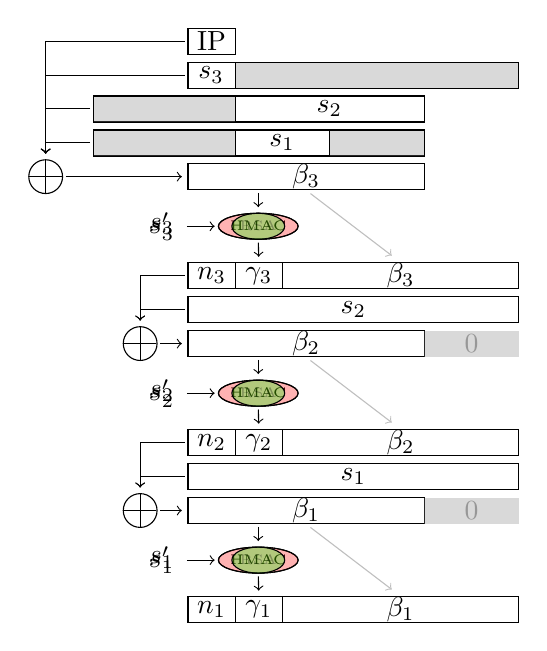
\begin{tikzpicture}
    \setlength{\y}{0cm}

    \node (ip) [block=1] at (0, \y) {IP};
    \vgap
    \node (s3_) [block=7] at (0, \y) {};
    \node [inblock=1] at (0, \y) {$s_3$};
    \node [inblock=6, gray] at (\width, \y) {}; 
    \vgap
    \node (s2_) [block=7] at (- 2*\width, \y) {};
    \node [inblock=3, gray] at (- 2*\width, \y) {}; 
    \node [inblock=4] at (3*\width - 2*\width, \y) {$s_2$}; 
    \vgap
    \node (s1_) [block=7] at (- 2*\width, \y) {};
    \node [inblock=3, gray] at (- 2*\width, \y) {}; 
    \node [inblock=2] at (3*\width - 2*\width, \y) {$s_1$};
    \node [inblock=2, gray] at (5*\width - 2*\width, \y) {};
    \vgap 
    \node (B3) [block=5] at (0, \y) {$\beta_3$}; 

    \node (xor3) [XOR] at (-3*\width, \y) {}; 
    \vGap
    \onslide <1-9> {\node (hmac3) [HMAC] at (1.5*\width, \y) {\tiny HMAC};}
    \onslide <2-9> {\node (hmac3) [HMAC, red] at (1.5*\width, \y) {\tiny HMAC};}
    \onslide <10-> {\node (hmac3) [HMAC, green] at (1.5*\width, \y) {\tiny RSA};}
    \vGap
 
    \node (n3) [block=1] at (0, \y) {$n_3$}; 
    \node (y3) [block=1] at (\width, \y) {$\gamma_3$}; 
    \node (b3) [block=5] at (2*\width, \y) {$\beta_3$}; 
    \vgap
    \node (s2) [block=7] at (0, \y) {$s_2$};
    \vgap
    \node (B2) [block=5] at (0, \y) {$\beta_2$}; 
    \node (zero2) [zero_pad=2] at (5*\width, \y) {0}; 

    \node (xor2) [XOR] at (-\width, \y) {}; 
    \vGap
    \onslide <1-9> {\node (hmac2) [HMAC] at (1.5*\width, \y) {\tiny HMAC};}
    \onslide <2-9> {\node (hmac2) [HMAC, red] at (1.5*\width, \y) {\tiny HMAC};}
    \onslide <10-> {\node (hmac2) [HMAC, green] at (1.5*\width, \y) {\tiny RSA};}
    \vGap

    \node (n2) [block=1] at (0, \y) {$n_2$}; 
    \node (y2) [block=1] at (\width, \y) {$\gamma_2$}; 
    \node (b2) [block=5] at (2*\width, \y) {$\beta_2$}; 
    \vgap
    \node (s1) [block=7] at (0, \y) {$s_1$};
    \vgap
    \node (B1) [block=5] at (0, \y) {$\beta_1$};
    \node (zero1) [zero_pad=2]  at (5*\width, \y) {0}; 

    \node (xor1) [XOR]  at (-\width, \y) {}; 
    \vGap
    \onslide <1-9> {\node (hmac1) [HMAC] at (1.5*\width, \y) {\tiny HMAC};}
    \onslide <2-9> {\node (hmac1) [HMAC, red] at (1.5*\width, \y) {\tiny HMAC};}
    \onslide <10-> {\node (hmac1) [HMAC, green] at (1.5*\width, \y) {\tiny RSA};}
    \vGap

    \node (n1) [block=1]  at (0, \y) {$n_1$}; 
    \node (y1) [block=1]  at (\width, \y) {$\gamma_1$}; 
    \node (b1) [block=5]  at (2*\width, \y) {$\beta_1$}; 

    %% XOR ARROWS %%
    % 3
    \draw[arrow] (ip.west) -- ++(-3*\width, 0) -- (xor3.north);
    \draw[arrow] (s3_.west) -- ++(-3*\width, 0) -- (xor3.north);
    \draw[arrow] (s2_.west) -- ++(-\width, 0) -- (xor3.north);
    \draw[arrow] (s1_.west) -- ++(-\width, 0) -- (xor3.north);
    \draw[arrow] (xor3.east) -- (B3.west);
    % 2
    \draw[arrow] (n3.west) -- ++(-\width, 0) -- (xor2.north);
    \draw[arrow] (s2.west) -- ++(-\width, 0) -- (xor2.north);
    \draw[arrow] (xor2.east) -- (B2.west);
    % 1
    \draw[arrow] (n2.west) -- ++(-\width, 0) -- (xor1.north);
    \draw[arrow] (s1.west) -- ++(-\width, 0) -- (xor1.north);
    \draw[arrow] (xor1.east) -- (B1.west);

    %% HMAC ARROWS %%
    % 3
    \onslide<1-9> {\node[left=\width of hmac3] (input_hmac3) {$s_3$};}
    \onslide<10-> {\node[left=\width of hmac3] (input_hmac3) {$s'_3$};}
    \draw[arrow, shorten >= 6pt] (input_hmac3) -- (hmac3.west);
    \draw[arrow] (B3.south -| 1.5*\width, 0) -- (hmac3.north);
    \draw[arrow] (hmac3.south) -- (y3.north);
    % 2
    \onslide<1-9> {\node[left=\width of hmac2] (input_hmac2) {$s_2$};}
    \onslide<10-> {\node[left=\width of hmac2] (input_hmac2) {$s'_2$};}
    \draw[arrow, shorten >= 6pt] (input_hmac2) -- (hmac2.west);
    \draw[arrow] (B2.south -| 1.5*\width, 0) -- (hmac2.north);
    \draw[arrow] (hmac2.south) -- (y2.north);
    % 1
    \onslide<1-9> {\node[left=\width of hmac1] (input_hmac1) {$s_1$};}
    \onslide<10-> {\node[left=\width of hmac1] (input_hmac1) {$s'_1$};}
    \draw[arrow, shorten >= 6pt] (input_hmac1) -- (hmac1.west);
    \draw[arrow] (B1.south -| 1.5*\width, 0) -- (hmac1.north);
    \draw[arrow] (hmac1.south) -- (y1.north);

    %% BETA ARROWS %%
    % 3
    \draw[arrowB] (B3.south) -- (b3.north);
    % 2
    \draw[arrowB] (B2.south) -- (b2.north);
    % 1
    \draw[arrowB] (B1.south) -- (b1.north);

\end{tikzpicture}
\end{column}

\end{columns}
\end{frame}
\begin{frame}{Adapting XOR}

\begin{columns} 
\small
\hspace{0.03\textwidth}
\begin{column}{0.47\textwidth}
    \onslide<3->
    Since we use \textbf{RSA} for integrity tag $\gamma_i$
    \onslide<4->
    \vspace{4mm}\newline
    $\begin{aligned}
        {\mathcal {E}}(m_{1}) {\color{green}\cdot} {\mathcal {E}}(m_{2})
        &=m_{1}^{e}m_{2}^{e}\;{\bmod {\;}}n\\[6pt]
        &=(m_{1}m_{2})^{e}\;{\bmod {\;}}n\\[6pt]
        &={\mathcal {E}}(m_{1} {\color{green}\cdot} m_{2})
    \end{aligned}$
    \onslide<5->
    \vspace{6mm}\newline
    {\color{green}Modular multiplication} of integrity tags gives integrity tag of headers’ {\color{green}modular product}.
    \onslide<6->
    \vspace{6mm}\newline
    \textbf{Thus, header elements must be combined via {\color{green}modular multiplication} rather than {\color{red}XOR}.}
\end{column}

\begin{column}{0.5\textwidth}
\onslide<1->
\centering
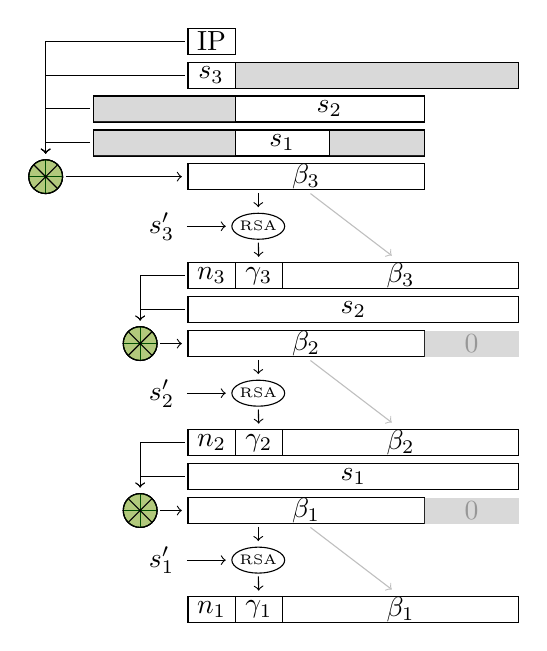
\begin{tikzpicture}
    \setlength{\y}{0cm}

    \node (ip) [block=1] at (0, \y) {IP};
    \vgap
    \node (s3_) [block=7] at (0, \y) {};
    \node [inblock=1] at (0, \y) {$s_3$};
    \node [inblock=6, gray] at (\width, \y) {}; 
    \vgap
    \node (s2_) [block=7] at (- 2*\width, \y) {};
    \node [inblock=3, gray] at (- 2*\width, \y) {}; 
    \node [inblock=4] at (3*\width - 2*\width, \y) {$s_2$}; 
    \vgap
    \node (s1_) [block=7] at (- 2*\width, \y) {};
    \node [inblock=3, gray] at (- 2*\width, \y) {}; 
    \node [inblock=2] at (3*\width - 2*\width, \y) {$s_1$};
    \node [inblock=2, gray] at (5*\width - 2*\width, \y) {};
    \vgap 
    \node (B3) [block=5] at (0, \y) {$\beta_3$}; 

    \onslide<1> {\node (xor3) [XOR] at (-3*\width, \y) {};}
    \onslide<2-5> {\node (xor3) [XOR, red] at (-3*\width, \y) {};} 
    \onslide<6-> {\node (xor3) [MULT, green] at (-3*\width, \y) {};}
    \vGap
    \node (hmac3) [HMAC] at (1.5*\width, \y) {\tiny RSA};
    \vGap
 
    \node (n3) [block=1] at (0, \y) {$n_3$}; 
    \node (y3) [block=1] at (\width, \y) {$\gamma_3$}; 
    \node (b3) [block=5] at (2*\width, \y) {$\beta_3$}; 
    \vgap
    \node (s2) [block=7] at (0, \y) {$s_2$};
    \vgap
    \node (B2) [block=5] at (0, \y) {$\beta_2$}; 
    \node (zero2) [zero_pad=2] at (5*\width, \y) {0}; 

    \onslide<1> {\node (xor2) [XOR] at (-\width, \y) {};}
    \onslide<2-5> {\node (xor2) [XOR, red] at (-\width, \y) {};} 
    \onslide<6-> {\node (xor2) [MULT, green] at (-\width, \y) {};}
    \vGap
    \node (hmac2) [HMAC] at (1.5*\width, \y) {\tiny RSA};
    \vGap

    \node (n2) [block=1] at (0, \y) {$n_2$}; 
    \node (y2) [block=1] at (\width, \y) {$\gamma_2$}; 
    \node (b2) [block=5] at (2*\width, \y) {$\beta_2$}; 
    \vgap
    \node (s1) [block=7] at (0, \y) {$s_1$};
    \vgap
    \node (B1) [block=5] at (0, \y) {$\beta_1$};
    \node (zero1) [zero_pad=2]  at (5*\width, \y) {0}; 

    \onslide<1> {\node (xor1) [XOR]  at (-\width, \y) {};}
    \onslide<2-5> {\node (xor1) [XOR, red] at (-\width, \y) {};} 
    \onslide<6-> {\node (xor1) [MULT, green] at (-\width, \y) {};}
    \vGap
    \node (hmac1) [HMAC]  at (1.5*\width, \y) {\tiny RSA};
    \vGap

    \node (n1) [block=1]  at (0, \y) {$n_1$}; 
    \node (y1) [block=1]  at (\width, \y) {$\gamma_1$}; 
    \node (b1) [block=5]  at (2*\width, \y) {$\beta_1$}; 

    %% XOR ARROWS %%
    % 3
    \draw[arrow] (ip.west) -- ++(-3*\width, 0) -- (xor3.north);
    \draw[arrow] (s3_.west) -- ++(-3*\width, 0) -- (xor3.north);
    \draw[arrow] (s2_.west) -- ++(-\width, 0) -- (xor3.north);
    \draw[arrow] (s1_.west) -- ++(-\width, 0) -- (xor3.north);
    \draw[arrow] (xor3.east) -- (B3.west);
    % 2
    \draw[arrow] (n3.west) -- ++(-\width, 0) -- (xor2.north);
    \draw[arrow] (s2.west) -- ++(-\width, 0) -- (xor2.north);
    \draw[arrow] (xor2.east) -- (B2.west);
    % 1
    \draw[arrow] (n2.west) -- ++(-\width, 0) -- (xor1.north);
    \draw[arrow] (s1.west) -- ++(-\width, 0) -- (xor1.north);
    \draw[arrow] (xor1.east) -- (B1.west);

    %% HMAC ARROWS %%
    % 3
    \node[left=\width of hmac3] (input_hmac3) {$s'_3$};
    \draw[arrow] (input_hmac3) -- (hmac3.west);
    \draw[arrow] (B3.south -| 1.5*\width, 0) -- (hmac3.north);
    \draw[arrow] (hmac3.south) -- (y3.north);
    % 2
    \node[left=\width of hmac2] (input_hmac2) {$s'_2$};
    \draw[arrow] (input_hmac2) -- (hmac2.west);
    \draw[arrow] (B2.south -| 1.5*\width, 0) -- (hmac2.north);
    \draw[arrow] (hmac2.south) -- (y2.north);
    % 1
    \node[left=\width of hmac1] (input_hmac1) {$s'_1$};
    \draw[arrow] (input_hmac1) -- (hmac1.west);
    \draw[arrow] (B1.south -| 1.5*\width, 0) -- (hmac1.north);
    \draw[arrow] (hmac1.south) -- (y1.north);

    %% BETA ARROWS %%
    % 3
    \draw[arrowB] (B3.south) -- (b3.north);
    % 2
    \draw[arrowB] (B2.south) -- (b2.north);
    % 1
    \draw[arrowB] (B1.south) -- (b1.north);

\end{tikzpicture}
\end{column}

\end{columns}
\end{frame}
\begin{frame}{Handle overflows}

\begin{columns} 
\small
\begin{column}{0.5\textwidth}
    \begin{itemize}
        \setlength\itemsep{5mm}
        \onslide<2->
        \item \textbf{Current Challenge:} \textbf{\color{red}Overflow} issues
        \onslide<3->
        \item Handling these issues is challenging.\newline
        It may lead to \textbf{information loss} \newline
        (further research is required).
        \onslide<4->
        \item \textbf{Proposed solution:} Simplify by \newline
        \textbf{\color{green}dividing data into small chunks} and \newline
        processing each chunk modulo its size. 
    \end{itemize}
\end{column}


\begin{column}{0.5\textwidth}
\onslide<1->
    \centering
    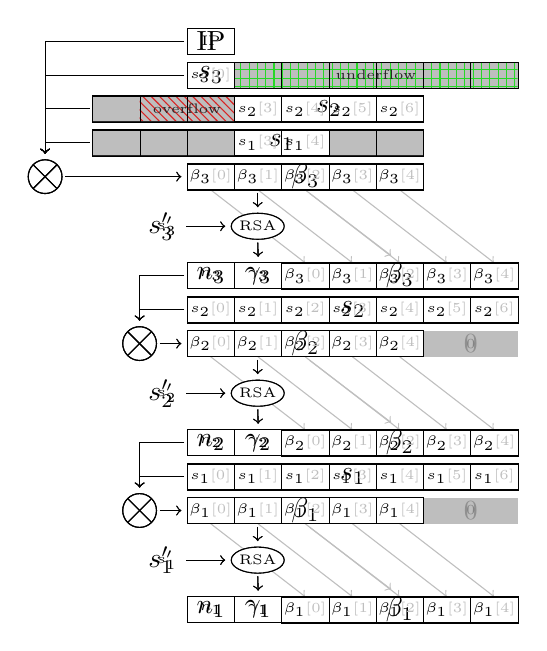
\begin{tikzpicture}
    \onslide<1-3> {
        \setlength{\y}{0cm}

        \node (ip) [block=1] at (0, \y) {IP};
        \vgap
        \node (s3_) [block=7] at (0, \y) {};
        \node [inblock=1] at (0, \y) {$s_3$};
        \node [inblock=6, gray] at (\width, \y) {}; 
        \onslide<2-> {\node [inblock=6, three] at (\width, \y) {\tiny underflow};}
        \vgap
        \node (s2_) [block=7] at (- 2*\width, \y) {};
        \node [inblock=3, gray] at (- 2*\width, \y) {}; 
        \node [inblock=4] at (3*\width - 2*\width, \y) {$s_2$}; 
        \onslide<2-> {\node [inblock=2, two] at (3*\width - 4*\width, \y) {\tiny overflow};}
        \vgap
        \node (s1_) [block=7] at (- 2*\width, \y) {};
        \node [inblock=3, gray] at (- 2*\width, \y) {}; 
        \node [inblock=2] at (3*\width - 2*\width, \y) {$s_1$};
        \node [inblock=2, gray] at (5*\width - 2*\width, \y) {};
        \vgap 
        \node (B3) [block=5] at (0, \y) {$\beta_3$}; 

        \node (xor3) [MULT] at (-3*\width, \y) {}; 
        \vGap
        \node (hmac3) [HMAC] at (1.5*\width, \y) {\tiny RSA};
        \vGap
    
        \node (n3) [block=1] at (0, \y) {$n_3$}; 
        \node (y3) [block=1] at (\width, \y) {$\gamma_3$}; 
        \node (b3) [block=5] at (2*\width, \y) {$\beta_3$}; 
        \vgap
        \node (s2) [block=7] at (0, \y) {$s_2$};
        \vgap
        \node (B2) [block=5] at (0, \y) {$\beta_2$}; 
        \node (zero2) [zero_pad=2] at (5*\width, \y) {0}; 

        \node (xor2) [MULT] at (-\width, \y) {}; 
        \vGap
        \node (hmac2) [HMAC] at (1.5*\width, \y) {\tiny RSA};
        \vGap

        \node (n2) [block=1] at (0, \y) {$n_2$}; 
        \node (y2) [block=1] at (\width, \y) {$\gamma_2$}; 
        \node (b2) [block=5] at (2*\width, \y) {$\beta_2$}; 
        \vgap
        \node (s1) [block=7] at (0, \y) {$s_1$};
        \vgap
        \node (B1) [block=5] at (0, \y) {$\beta_1$};
        \node (zero1) [zero_pad=2]  at (5*\width, \y) {0}; 

        \node (xor1) [MULT]  at (-\width, \y) {}; 
        \vGap
        \node (hmac1) [HMAC]  at (1.5*\width, \y) {\tiny RSA};
        \vGap

        \node (n1) [block=1]  at (0, \y) {$n_1$}; 
        \node (y1) [block=1]  at (\width, \y) {$\gamma_1$}; 
        \node (b1) [block=5]  at (2*\width, \y) {$\beta_1$}; 

        %% XOR ARROWS %%
        % 3
        \draw[arrow] (ip.west) -- ++(-3*\width, 0) -- (xor3.north);
        \draw[arrow] (s3_.west) -- ++(-3*\width, 0) -- (xor3.north);
        \draw[arrow] (s2_.west) -- ++(-\width, 0) -- (xor3.north);
        \draw[arrow] (s1_.west) -- ++(-\width, 0) -- (xor3.north);
        \draw[arrow] (xor3.east) -- (B3.west);
        % 2
        \draw[arrow] (n3.west) -- ++(-\width, 0) -- (xor2.north);
        \draw[arrow] (s2.west) -- ++(-\width, 0) -- (xor2.north);
        \draw[arrow] (xor2.east) -- (B2.west);
        % 1
        \draw[arrow] (n2.west) -- ++(-\width, 0) -- (xor1.north);
        \draw[arrow] (s1.west) -- ++(-\width, 0) -- (xor1.north);
        \draw[arrow] (xor1.east) -- (B1.west);

        %% HMAC ARROWS %%
        % 3
        \node[left=\width of hmac3] (input_hmac3) {$s'_3$};
        \draw[arrow] (input_hmac3) -- (hmac3.west);
        \draw[arrow] (B3.south -| 1.5*\width, 0) -- (hmac3.north);
        \draw[arrow] (hmac3.south) -- (y3.north);
        % 2
        \node[left=\width of hmac2] (input_hmac2) {$s'_2$};
        \draw[arrow] (input_hmac2) -- (hmac2.west);
        \draw[arrow] (B2.south -| 1.5*\width, 0) -- (hmac2.north);
        \draw[arrow] (hmac2.south) -- (y2.north);
        % 1
        \node[left=\width of hmac1] (input_hmac1) {$s'_1$};
        \draw[arrow] (input_hmac1) -- (hmac1.west);
        \draw[arrow] (B1.south -| 1.5*\width, 0) -- (hmac1.north);
        \draw[arrow] (hmac1.south) -- (y1.north);

        %% BETA ARROWS %%
        % 3
        \draw[arrowB] (B3.south) -- (b3.north);
        % 2
        \draw[arrowB] (B2.south) -- (b2.north);
        % 1
        \draw[arrowB] (B1.south) -- (b1.north);
    }
    \onslide<4-> {
        \tiny
        \setlength{\y}{0cm}

        \node (ip) [block=1] at (0, \y) {IP};
        \vgap
        \node (s3_) [block=7] at (0, \y) {};
        \node [inblock=1] at (0, \y) {$s_3{\textcolor{lightgray}{[0]}}$};
        \foreach \i in {1,...,6} {
            \node [inblock=1, gray] at (\i*\width, \y) {}; 
        }
        \vgap
        \node (s2_) [block=7] at (- 2*\width, \y) {};
        \foreach \i in {0,...,2} {
            \node [inblock=1, gray] at (-\i*\width, \y) {}; 
        } 
        \foreach \i in {3,...,6} {
            \node [inblock=1] at (\i*\width - 2*\width, \y) {$s_2{\textcolor{lightgray}{[\i]}}$}; 
        }
        \vgap
        \node (s1_) [block=7] at (- 2*\width, \y) {};
        \foreach \i in {0,...,2} {
            \node [inblock=1, gray] at (-\i*\width, \y) {}; 
        }
        \foreach \i in {3,...,4} {
            \node [inblock=1] at (\i*\width - 2*\width, \y) {$s_1{\textcolor{lightgray}{[\i]}}$}; 
        }
        \foreach \i in {3,...,4} {
            \node [inblock=1, gray] at (\i*\width, \y) {}; 
        }
        \vgap 
        \foreach \i in {0,...,4} {
            \node (B3\i) [inblock=1] at (\i*\width, \y) {$\beta_3{\textcolor{lightgray}{[\i]}}$}; 
        }
        \node (xor3) [MULT] at (-3*\width, \y) {}; 
        \vGap
        \node (hmac3) [HMAC, fill=white] at (1.5*\width, \y) {\tiny RSA};
        \vGap
    
        \node (n3) [block=1] at (0, \y) {$n_3$}; 
        \node (y3) [block=1] at (\width, \y) {$\gamma_3$}; 
        \foreach \i in {0,...,4} {
            \node (b3\i) [inblock=1] at (2*\width + \i*\width, \y) {$\beta_3{\textcolor{lightgray}{[\i]}}$}; 
        }
        \vgap
        \foreach \i in {0,...,6} {
            \node (s2\i) [inblock=1] at (\i*\width, \y) {$s_2{\textcolor{lightgray}{[\i]}}$};
        }
        \vgap
        \foreach \i in {0,...,4} {
            \node (B2\i) [inblock=1] at (\i*\width, \y) {$\beta_2{\textcolor{lightgray}{[\i]}}$}; 
        }
        \node (zero2) [zero_pad=2] at (5*\width, \y) {0}; 

        \node (xor2) [MULT] at (-\width, \y) {}; 
        \vGap
        \node (hmac2) [HMAC, fill=white] at (1.5*\width, \y) {\tiny RSA};
        \vGap

        \node (n2) [block=1] at (0, \y) {$n_2$}; 
        \node (y2) [block=1] at (\width, \y) {$\gamma_2$}; 
        \foreach \i in {0,...,4} {
            \node (b2\i) [inblock=1] at (2*\width + \i*\width, \y) {$\beta_2{\textcolor{lightgray}{[\i]}}$}; 
        }
        \vgap
        \foreach \i in {0,...,6} {
            \node (s1\i) [inblock=1] at (\i*\width, \y) {$s_1{\textcolor{lightgray}{[\i]}}$};
        }    
        \vgap
        \foreach \i in {0,...,4} {
            \node (B1\i) [inblock=1] at (\i*\width, \y) {$\beta_1{\textcolor{lightgray}{[\i]}}$};
        }
        \node (zero1) [zero_pad=2]  at (5*\width, \y) {0}; 

        \node (xor1) [MULT]  at (-\width, \y) {}; 
        \vGap
        \node (hmac1) [HMAC, fill=white]  at (1.5*\width, \y) {\tiny RSA};
        \vGap

        \node (n1) [block=1]  at (0, \y) {$n_1$}; 
        \node (y1) [block=1]  at (\width, \y) {$\gamma_1$}; 
        \foreach \i in {0,...,4} {
            \node (b1\i) [inblock=1]  at (2*\width + \i*\width, \y) {$\beta_1{\textcolor{lightgray}{[\i]}}$}; 
        }

        %% XOR ARROWS %%
        % 3
        \draw[arrow] (ip.west) -- ++(-3*\width, 0) -- (xor3.north);
        \draw[arrow] (s3_.west) -- ++(-3*\width, 0) -- (xor3.north);
        \draw[arrow] (s2_.west) -- ++(-\width, 0) -- (xor3.north);
        \draw[arrow] (s1_.west) -- ++(-\width, 0) -- (xor3.north);
        \draw[arrow] (xor3.east) -- (B3.west);
        % 2
        \draw[arrow] (n3.west) -- ++(-\width, 0) -- (xor2.north);
        \draw[arrow] (s2.west) -- ++(-\width, 0) -- (xor2.north);
        \draw[arrow] (xor2.east) -- (B2.west);
        % 1
        \draw[arrow] (n2.west) -- ++(-\width, 0) -- (xor1.north);
        \draw[arrow] (s1.west) -- ++(-\width, 0) -- (xor1.north);
        \draw[arrow] (xor1.east) -- (B1.west);

        %% HMAC ARROWS %%
        % 3
        \node[left=\width of hmac3] (input_hmac3) {$s'_3$};
        \draw[arrow] (input_hmac3) -- (hmac3.west);
        \draw[arrow] (B3.south -| 1.5*\width, 0) -- (hmac3.north);
        \draw[arrow] (hmac3.south) -- (y3.north);
        % 2
        \node[left=\width of hmac2] (input_hmac2) {$s'_2$};
        \draw[arrow] (input_hmac2) -- (hmac2.west);
        \draw[arrow] (B2.south -| 1.5*\width, 0) -- (hmac2.north);
        \draw[arrow] (hmac2.south) -- (y2.north);
        % 1
        \node[left=\width of hmac1] (input_hmac1) {$s'_1$};
        \draw[arrow] (input_hmac1) -- (hmac1.west);
        \draw[arrow] (B1.south -| 1.5*\width, 0) -- (hmac1.north);
        \draw[arrow] (hmac1.south) -- (y1.north);

        %% BETA ARROWS %%
        \begin{pgfonlayer}{background}
            % 3
            \foreach \i in {0,...,4} {
                \draw[->, color=lightgray] (B3\i.south) -- (b3\i.north);
            }
            % 2
            \foreach \i in {0,...,4} {
                \draw[->, color=lightgray] (B2\i.south) -- (b2\i.north);
            }
            % 1
            \foreach \i in {0,...,4} {
                \draw[->, color=lightgray] (B1\i.south) -- (b1\i.north);
            }
        \end{pgfonlayer}
    }
    \end{tikzpicture}
\end{column}

\end{columns}
\end{frame}

\end{document}
